\documentclass[a4paper,11pt]{article}
\usepackage{amsmath,amsthm,amsfonts,amssymb,amscd,amstext,vmargin,graphics,graphicx,tabularx,multicol} 
\usepackage[francais]{babel}
\usepackage[utf8]{inputenc}  
\usepackage[T1]{fontenc} 
\usepackage{pstricks-add,tikz,tkz-tab,variations}
\usepackage[autolanguage,np]{numprint} 

\setmarginsrb{1.5cm}{0.5cm}{1cm}{0.5cm}{0cm}{0cm}{0cm}{0cm} %Gauche, haut, droite, haut
\newcounter{numexo}
\newcommand{\exo}[1]{\stepcounter{numexo}\noindent{\bf Exercice~\thenumexo} : \marginpar{\hfill /#1}}
\reversemarginpar


\newcounter{enumtabi}
\newcounter{enumtaba}
\newcommand{\q}{\stepcounter{enumtabi} \theenumtabi.  }
\newcommand{\qa}{\stepcounter{enumtaba} (\alph{enumtaba}) }
\newcommand{\initq}{\setcounter{enumtabi}{0}}
\newcommand{\initqa}{\setcounter{enumtaba}{0}}

\newcommand{\be}{\begin{enumerate}}
\newcommand{\ee}{\end{enumerate}}
\newcommand{\bi}{\begin{itemize}}
\newcommand{\ei}{\end{itemize}}
\newcommand{\bp}{\begin{pspicture*}}
\newcommand{\ep}{\end{pspicture*}}
\newcommand{\bt}{\begin{tabular}}
\newcommand{\et}{\end{tabular}}
\renewcommand{\tabularxcolumn}[1]{>{\centering}m{#1}} %(colonne m{} centrée, au lieu de p par défault) 
\newcommand{\tnl}{\tabularnewline}

\newcommand{\bmul}[1]{\begin{multicols}{#1}}
\newcommand{\emul}{\end{multicols}}

\newcommand{\trait}{\noindent \rule{\linewidth}{0.2mm}}
\newcommand{\hs}[1]{\hspace{#1}}
\newcommand{\vs}[1]{\vspace{#1}}

\newcommand{\N}{\mathbb{N}}
\newcommand{\Z}{\mathbb{Z}}
\newcommand{\R}{\mathbb{R}}
\newcommand{\C}{\mathbb{C}}
\newcommand{\Dcal}{\mathcal{D}}
\newcommand{\Ccal}{\mathcal{C}}
\newcommand{\mc}{\mathcal}

\newcommand{\vect}[1]{\overrightarrow{#1}}
\newcommand{\ds}{\displaystyle}
\newcommand{\eq}{\quad \Leftrightarrow \quad}
\newcommand{\vecti}{\vec{\imath}}
\newcommand{\vectj}{\vec{\jmath}}
\newcommand{\Oij}{(O;\vec{\imath}, \vec{\jmath})}
\newcommand{\OIJ}{(O;I,J)}


\newcommand{\reponse}[1][1]{%
\multido{}{#1}{\makebox[\linewidth]{\rule[0pt]{0pt}{20pt}\dotfill}
}}

\newcommand{\titre}[5] 
% #1: titre #2: haut gauche #3: bas gauche #4: haut droite #5: bas droite
{
\noindent #2 \hfill #4 \\
#3 \hfill #5

\vspace{-1.6cm}

\begin{center}\rule{6cm}{0.5mm}\end{center}
\vspace{0.2cm}
\begin{center}{\large{\textbf{#1}}}\end{center}
\begin{center}\rule{6cm}{0.5mm}\end{center}
}



\begin{document}
\pagestyle{empty}
\titre{Interrogation: Les angles }{Nom :}{Prénom :}{Classe}{Date}


\begin{tabular}{|m{11cm}|c|c|c|}
\hline 
\textbf{Compétences} & \textbf{Acquis} & \textbf{En cours}  & \textbf{Non acquis} \\ 
\hline 
- Connaître le vocabulaire (sommet, côtés) et les notations associées &  &  & \\
\hline
- Connaitre le vocabulaire (nul, aigu, droit, obtus, plat)&  &  &  \\ 
\hline
- Mesurer un angle en degré (avec un rapporteur). &  &  &  \\ 
\hline 
- Construire un angle de mesure donnée en degré (avec un rapporteur).  &  &  &  \\ 
\hline 

- Savoir définir une bissectrice et savoir construire la bissectrice d'un angle.  &  &  &  \\ 
\hline 

\end{tabular} 

\vspace*{0.5cm}

\exo{3,5} Cours \\

\q Donner la définition d'une bissectrice.\\
\reponse[2]\\

\bmul{2}
\q  Compléter : \\

- L'angle  $\widehat{xAB}$ est formé par les demi-droites   . . . .  et . . . . . . \\


\q  Sur la figure, colorier en rouge  l'angle  $\widehat{CAz}$ , en bleu l'angle $\widehat{uBA}$ en vert l'angle $\widehat{yCB}$  et en noir l'angle $\widehat{xAz}$.\\

\q Construire ci-dessous l'angle $\widehat{TAL} = 78$\degre et construire [AI) la bissectrice de l'angle $\widehat{TAL} $.\\

\columnbreak

\begin{flushright}
\includegraphics[scale=0.95]{cours.eps} 

\end{flushright}
\emul



\vspace*{3.5cm}

\exo{3,5}

\begin{flushleft}
\includegraphics[scale=0.9]{tableauinterro.eps} \\

\end{flushleft}

\newpage


\exo{1,5} (Attention la figure est volontairement fausse.)

\begin{center}
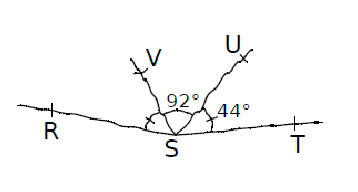
\includegraphics[scale=1]{alignes.eps} 
\end{center}


Les points R, S et T sont-ils alignés? \textbf{Justifier} votre réponse à l'aide de votre cours.\\
\reponse[5]\\

\exo{1,5} Cassiopée est une des 88 constellations du ciel. Voici des indications pour réaliser un plan de cette constellation.

\begin{center}
\includegraphics[scale=1]{cassiopeeangles.eps} 
\end{center}

Reproduire ci-dessous la construction de ce plan en vraie grandeur.



\end{document}
